\begin{figure}[t]
    \centering
    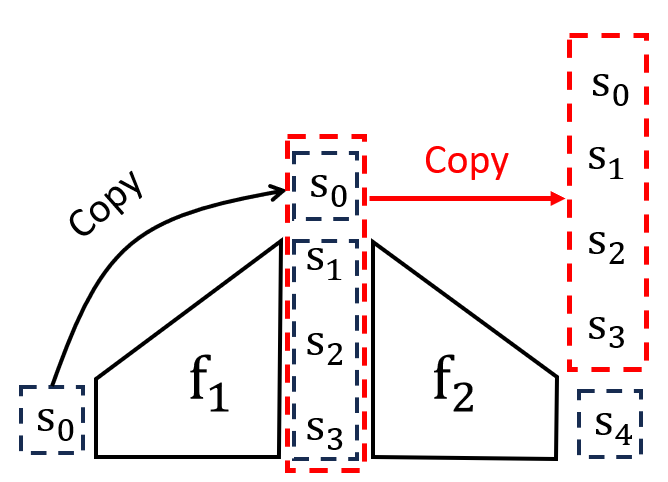
\includegraphics[width=0.5\linewidth]{figures/Method.PNG}
    \caption{Shows the methodology to combine $\dynamics_1$ and $\dynamics_2$ in order to map the initial state to the trajectory with a feed forward neural network. We use linear activation function to copy the states.}
    \label{fig:method}
\end{figure}
\subsection{Training the Model} \label{apdx:training}

\noindent Defining the set of sub-horizons as,
 $
 \Pi = \left\{\pi_1\!\!=\!\!1,  \pi_2,...,\pi_v \right\}\!\! \subset\!\! \mathbb{N}$,  $ \theta_j=\sum_{i=1}^j \pi_i , \theta_0=0,\theta_{v} = \horizon+1 
 $, then, for a given $j\in [v-1]$ , we decompose the training dataset $D_{\text{train}}$ as follows:
 $$
 \begin{aligned}
 &D_{\text{train}}^j = \left\{ 
 \mathsf{feature\!\!-\!\!data}(j,\ell), \mathsf{target\!\!-\!\!data}(j,\ell)
 \right\}_{\ell=1}^L,\\
 &\mathsf{feature\!\!-\!\!data}(j,\ell) =  
 \left\{ \traj_{\state_0^\ell}(\theta_{j-1}+i)\right\}_{i=0}^{\pi_{j}-1}, \\
 &\mathsf{target\!\!-\!\!data}(j,\ell) = \left\{ \traj_{\state_0^\ell}(\theta_{j}+i)\right\}_{i=0}^{\pi_{j+1}-1},
 \end{aligned}
 $$
 our approach is based on training a set of different models like, $\dynamics_j: \mathbb{R}^{\pi_j n} \to \mathbb{R}^{\pi_{j+1} n}, $ over $D_{\text{train}}^j, j\in [v-1]$, to be combined in order to generate a map, $\overallf: \mathbb{R}^n \to \mathbb{R}^{(\horizon+1) n}$, between initial state, $\state_0 \in \mathbb{R}^n$ and trajectory predictions $\bar{\traj}_{\state_0}$,
 $$
 \bar{\traj}_{\state_0} = \overallf(\state_0).
 $$
\mypara{Example:} We sample $L=3$ initial states with dimension $n=1$ as, $\state_0^1=1, \state_0^2=2, \state_0^3=1, $ and using a pre-defined stochastic feedback policy we generate three $\horizon$-step trajectories with $\horizon =4$ as follows:
$$
\traj_{\state_0^1} = \left\{ 1, 3, 5, 2,3 \right\}, \traj_{\state_0^2} = \left\{ 2, 4, 6, 3,4 \right\},  \traj_{\state_0^3} = \left\{ 1, 3, 4, 2,4 \right\}.
$$
We want to train two models $\dynamics_1: \mathbb{R}^1 \to \mathbb{R}^3$, $\dynamics_2: \mathbb{R}^3 \to \mathbb{R}^1$. Therefore, we define the set of sub-horizons $\Pi=\left\{1,3,1 \right\}$. Thus the feature and target dataset for $\dynamics_1$ is:
$$
\begin{aligned}
&\mathsf{feature\!\!-\!\!data}(1,[1,2,3])=\left\{\left\{1\right\},\left\{2\right\},\left\{1\right\} \right\}\\
&\mathsf{target\!\!-\!\!data}(1,[1,2,3])=\left\{ \left\{3,5,2\right\},\left\{4,6,3\right\},\left\{3,5,2\right\} \right\}
\end{aligned}
$$
and the feature and target dataset for $\dynamics_2$ is:
$$
\begin{aligned}
&\mathsf{feature\!\!-\!\!data}(2,[1,2,3])=\left\{ \left\{3,5,2\right\},\left\{4,6,3\right\},\left\{3,5,2\right\} \right\}\\
&\mathsf{target\!\!-\!\!data}(2,[1,2,3])=\left\{\left\{3\right\},\left\{4\right\},\left\{4\right\} \right\}
\end{aligned}
$$
we then combine $\dynamics_1$ and $\dynamics_2$ such that, the combined model, $\overallf$, receives the initial state and predicts all the trajectory. Figure \ref{fig:method} shows the method we utilized to combine them.


